\section{Feature Extraction}
\label{sec:feature_extraction}

Feature extraction is one of the key steps in all supervised learning problems. The resulting feature vector (in numeric form) of the feature extraction step is fed as an input into machine learning algorithms (K-NN, SVM, NB, etc.) for the construction and validation of classification/regression model~\cite{jahangir:review}.

Short-term spectral features are extracted from short frames (\num{20} - \SI{30}{ms}) of speech signals, as the speech signal changes continuously due to the articulation of sounds. As a result of these short frames, the extracted features are perceived to be stationary and preserve the local information. Mel Frequency Cepstral Coefficients (MFCCs) and Linear Predictor Cepstral Coefficients (LPCCs) are the most widely employed short-term spectral features in speaker identification~\cite{jahangir:review}, indeed we could say that cepstral coefficients derived from either linear prediction analysis or a filter bank approach are today still considered the de-facto standard in the audio feature extraction~\cite{rao:spectral}, even if many deep learning-related works \cite{si:sincnet}, \cite{si:lstm}, \cite{si:cnn} have shown how less refined features (raw waveform signals, raw log-spectrograms or Mel-scaled log-spectrum features, ...) can also be just as effective if not better in some cases.

It's important to note that one of the reasons for such success is that spectral features represent phonetic information, since they are derived directly from spectra~\cite{rao:spectral}, and these are the ones that allow a better discerning between speakers. In the next two sections we go in more details about the two aforementioned coefficients and how we used them in our study.

\subsection{MFCCs}
Mel Frequency Cepstral Coefficents (MFCCs) are widely used features in ASR and SI. They were introduced by Davis and Mermelstein in the '80s, and have been state-of-the-art ever since.

As the name suggests, MFCCs are based on the Mel-scale (where \textit{Mel} stands for \textit{melody}), a logarithmic scale devised to map the frequency of a sound on a scale that better reflects the human perception of them. Figure \vref{fig:mel_hz_plot} shows the plot of pitch Mel scale versus Hertz scale, we can note how \SI{1000}{mel} equals \SI{1000}{Hz}.

\begin{figure}
	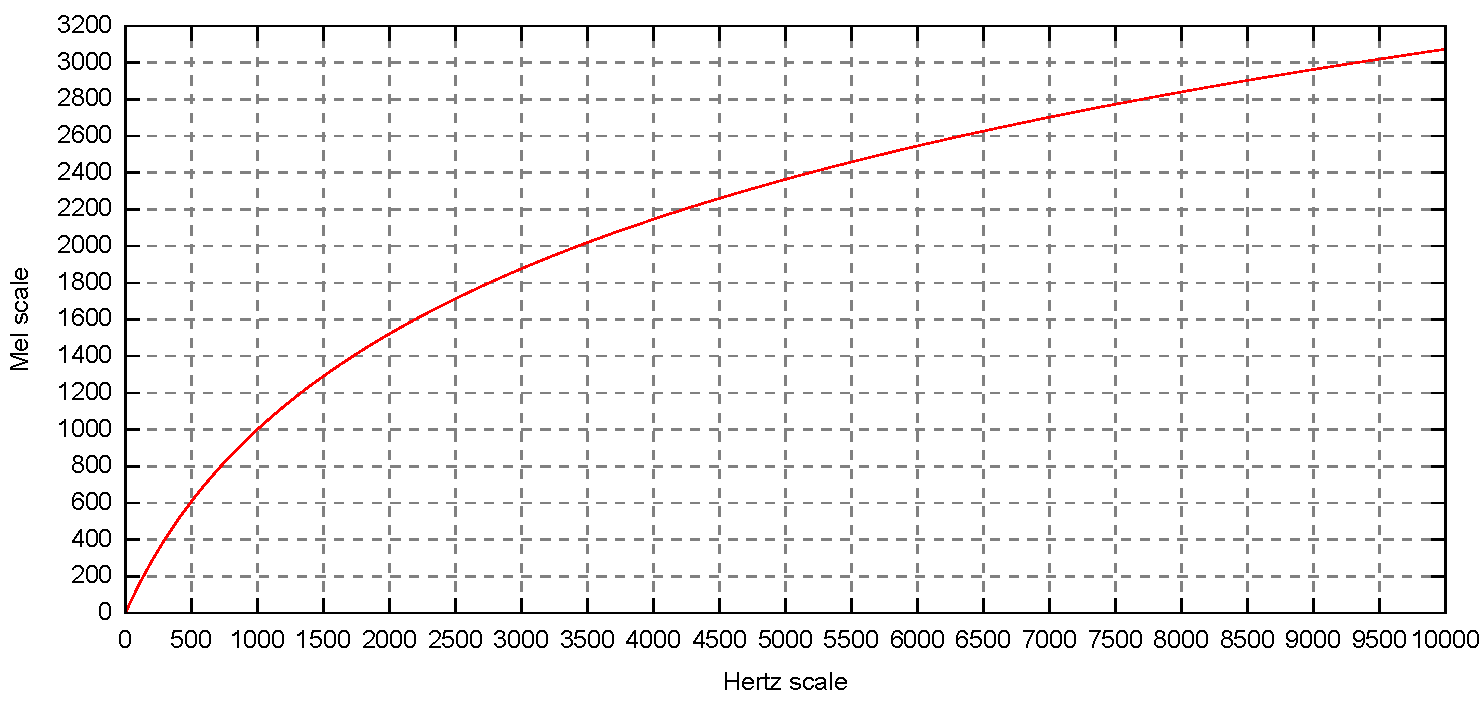
\includegraphics[width=0.5\textwidth]{images/mel_hz_plot}
	\caption{Plot of pitch mel scale versus Hertz scale, source~\cite{wiki:mel_scale}.}
	\label{fig:mel_hz_plot}
\end{figure}

The MFCC feature extraction technique basically includes windowing the signal, applying the DFT, taking the log of the magnitude, and then warping the frequencies on a Mel scale, followed by applying the inverse DCT. The detailed description of the various steps involved in the MFCC feature extraction is explained below.

\subsubsection{Pre-Emphasis}
Pre-emphasis refers to filtering that emphasizes the higher frequencies. It is used to balance the spectrum of voiced sounds that have a steep drop in the high frequency range. Usually the glottal source has a slope of about -12 dB/octave. However, when acoustic energy is radiated from the lips, this results in a spectrum rise of about +6 dB/octave. Therefore, pre-distortion removes some of the glottal effects from the vocal tract parameters.

The most commonly used pre-emphasis filter is given by the following transfer function:
$$
H(z)=1-b z^{-1}
$$

\subsubsection{Framing}
The speech signal is a slowly time-varying or quasi-stationary signal. For stable acoustic characteristics, speech needs to be examined over a sufficiently short period of time. Therefore, speech analysis must always be carried out on short segments across which the speech signal is assumed to be stationary; usually, it is divided into smaller frames each lasting between 20ms and 40ms.

\subsubsection{Windowing}
Advancing the time window every 10 ms enables the temporal characteristics of individual speech sounds to be tracked, and the 20 ms analysis window is usually sufficient to provide good spectral resolution of these sounds, and at the same time short enough to resolve significant temporal characteristics. The purpose of the overlapping analysis is that each speech sound of the input sequence would be approximately centered at some frame. On each frame, a window is applied to taper the signal towards the frame boundaries. This is done to enhance the harmonics, smooth the edges, and to reduce the edge effect while taking the DFT on the signal.
Hamming window has been used as window shape by considering the next block in feature extraction processing chain and integrates all the closest frequency lines. Let:
\begin{itemize}
    \item $X_n$ = input signal;
    \item $Y_n$ = output signal;
    \item $W_n$ = hamming window;
\end{itemize}
then the resulting windowed signal is:
\begin{center}
$Y_n = X_n \times W_n, \quad n=0,1,2,\ldots,N$
\end{center}

\paragraph{DFT Spectrum}
Each windowed frame is converted into magnitude spectrum by applying DFT.
$$
X(k)=\sum_{n=0}^{N-1} x(n) e^{\frac{-j 2 \pi n k}{N}} ; \quad 0 \leq k \leq N-1
$$

\subsubsection{Mel Spectrum}
Mel spectrum is computed by passing the Fourier-transformed signal through a set of band-pass filters known as Mel-filter bank. A Mel is a unit of measure based on the human ears perceived frequency. It does not correspond linearly to the physical frequency of the tone, as the human auditory system apparently does not perceive pitch linearly~\cite{rao:spectral}. We reported the relationship between Mel-scale and Hertz-scale in figure \vref{fig:mel_hz_plot}. The approximation of Mel from physical frequency can be expressed as:
\begin{equation}\label{eq:1}
	f_{\Mel}=2595 \log _{10}\left(1+\frac{f}{700}\right)
\end{equation}
where $f$ denotes the physical frequency in Hz, and $f_{\Mel}$ denotes the perceived frequency~\cite{deller:dt_processing}.

Filter banks can be implemented in either the time domain or the frequency domain, but in MFCC computation, they are usually implemented in the latter one. The center frequencies of the filters are normally evenly spaced on the frequency axis, however, to mimic the perception of the human ear, a warped axis is implemented, according to the nonlinear function given in eq. \vref{eq:1}. The most commonly used filter shaper is triangular, the triangular filter banks with Mel frequency warping we used is presented in figure \vref{fig:mel_filter_bank}.
\begin{figure}
  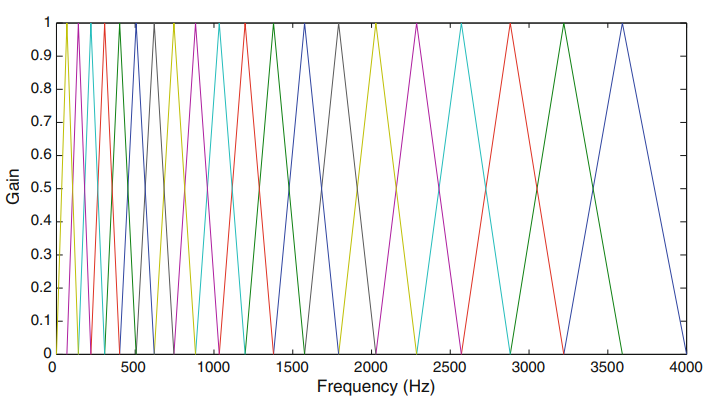
\includegraphics[width=0.5\textwidth]{images/mel_filters.png}
  \caption{Mel-filter bank, source~\cite{rao:spectral}}.
  \label{fig:mel_filter_bank}
\end{figure}

The Mel spectrum of the magnitude spectrum $X(k)$ is computed by multiplying the magnitude spectrum by each of the triangular Mel weighting filters:
\begin{equation}\label{eq:2}
s(m)=\sum_{k=0}^{N-1}\left[ \lvert X(k) \rvert ^{2} H_{m}(k)\right] ; \quad 0 \leq m \leq M-1
\end{equation}
where $M$ is the total number of triangular Mel weighting filters. $H_{m}(k)$ is the weight given to the $k$-th energy spectrum bin contributing to the $m$-th output band and is expressed as~\cite{rao:spectral}:
\begin{equation}
	H_{m}(k)=\left\{\begin{array}{cl}
	0, & k<f(m-1) \\ \\
	\frac{2(k-f(m-1))}{f(m)-f(m-1)}, & f(m-1) \leq k \leq f(m) \\ \\
	\frac{2(f(m+1)-k)}{f(m+1)-f(m)}, & f(m)<k \leq f(m+1) \\ \\
	0, & k>f(m+1)
	\end{array}\right.
\end{equation}

\subsubsection{Discrete Cosine Transform}

Since the vocal tract is smooth, the energy levels in adjacent bands tend to be correlated. Before computing the DCT, the Mel spectrum is usually represented on a log scale, then DCT is applied to the transformed mel frequency coefficients to produce a set of cepstral coefficients. This results in a signal in the cepstral domain with a quefrency peak corresponding to the pitch of the signal and a number of formants representing low quefrency peaks~\cite{rao:spectral}.

Since most of the signal information (corresponding to the vocal tract features) is represented by the first few MFCC coefficients, we only selected the first 13, as usual in most literature. As in~\cite{picone:signal_modeling}, extracting only those coefficients ignoring or truncating higher order DCT components is sufficient to obtain a robust system. Finally we report, again from~\cite{picone:signal_modeling}, the final formula for calculating MFCCs involving DCT:
\begin{equation}
	c(n)=\sum_{m=0}^{M-1} \log _{10}(s(m)) \cos \left(\frac{\pi n(m-0.5)}{M}\right)
\end{equation}
with $n=0,1,2, \ldots, C-1$, where $c(n)$ are the cepstral coefficients and $C$ is the number of MFCCs, usually between \num{8} and \num{13}.

\subsubsection{First and Second Order Derivatives}
First and second derivative of each MFCC (also known as delta and delta-delta features) are also taken into account, since they carry additional information about the coefficient variation over time, ending up with 39 coefficients for each frame, which will become the input of our deep learning model.

Delta coefficients tell about the speech rate, while delta-delta coefficients provide information similar to acceleration of speech~\cite{rao:spectral}. The commonly used definition for computing these dynamic parameters (delta features) is:
\begin{equation}
	\Delta c_m(n) = \frac{\sum_{i = -T}^{T} k_i c_m (n + i)}{\sum_{i = -T}^{T}\lvert i \rvert}
\end{equation}
where $c_m(n)$ denotes the $m$-th feature for the $n$-th time frame, $k_i$ is the $i$-th weight and $T$ is the number of successive frames used for computation. Generally $T$ is taken as $2$. The delta-delta coefficients are computed by taking the first order derivative of the delta coefficients~\cite{rao:spectral}.

\subsection{LPCCs}
LPCCs are another type of cepstral coefficients widely used in speech processing~\cite{jahangir:review}. As mentioned in the section~\vref{sec:feature_extraction}, spectral features represent phonetic information, as they are derived directly from spectra. The features extracted from spectra, using the energy values of linearly arranged filter banks, equally emphasize the contribution of all frequency components of a speech signal. In this context, LPCCs are used to capture emotion-specific information manifested through vocal tract features~\cite{rao:spectral}.

As in the case of MFCCs, the Linear Predictive (LP) analysis requires multiple steps, exemplified in the figure \vref{fig:lpc}, that represents the steps from the speech signal to the LPCs (Linear Predictive Coefficients). The next step is to actually extract the cepstral coefficients, as shown in Figure~\vref{fig:lpcc}.
\begin{figure}
	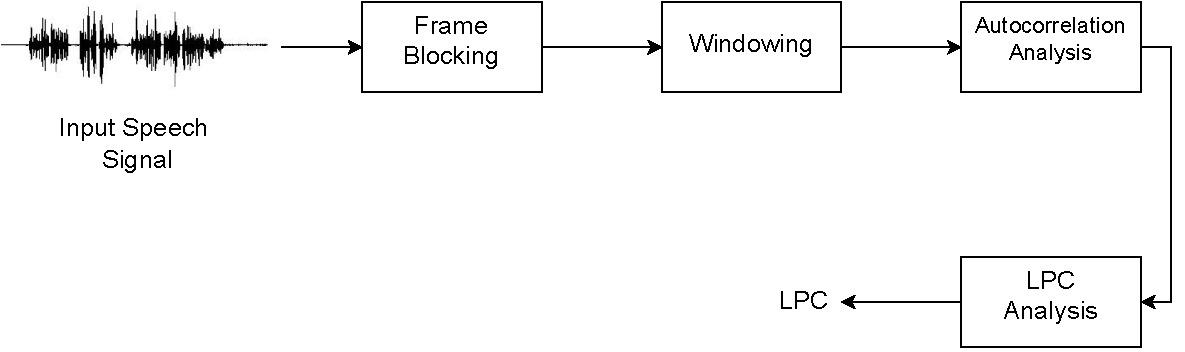
\includegraphics[width=0.5\textwidth]{images/lpc}
	\caption{LPC block diagram.}
	\label{fig:lpc}
\end{figure}
\begin{figure}
	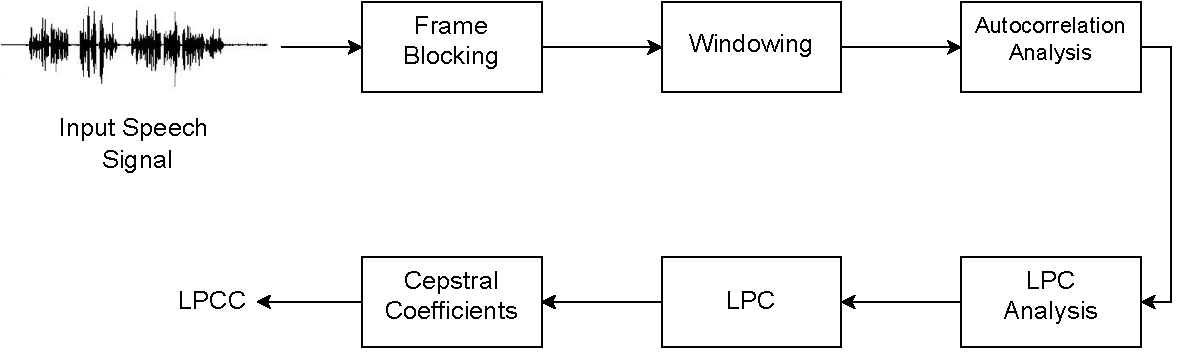
\includegraphics[width=0.5\textwidth]{images/lpcc}
	\caption{LPCC block diagram.}
	\label{fig:lpcc}
\end{figure}

In this work we extracted from the speech signal 13 LPCCs per speech frame of \SI{16}{ms}, using an overlap of \SI{8}{ms} and the \textit{hann} windowing.

\subsubsection{Cepstrum and LPCCs Calculation}

Cepstrum may be obtained using linear prediction analysis of a speech signal. The basic idea behind linear predictive analysis is that the $n$th speech sample can be
estimated by a linear combination of its previous $p$ samples as shown in the following equation~\cite{rao:spectral}:

\begin{multline}
	s(n) \thickapprox a_1s(n - 1) + a_2s(n - 2) +\\+ a_3s(n - 3) + \dots + a_ps(n - p)
\end{multline}
where $a_1, a_2, a_3, \dots$ are assumed to be constants over a speech analysis frame. These are known as predictor coefficients or linear predictive coefficients. These coefficients are used to predict the speech samples, then we can calculate the error as the difference of actual and predicted speech samples, by the following formula:

\begin{equation}
	e(n) = s(n) - \hat{s}(n) = s(n) - \sum_{k = 1}^{p}a_ks(n - k)
\end{equation}
where $e(n)$ is the error in prediction, $s(n)$ is the original speech signal, $\hat{s}(n)$ is a predicted speech signal and $a_k$s are the predictor coefficients.

To compute a unique set of predictor coefficients, the sum of squared differences between the actual and predicted speech samples has to be minimized (error minimization) as shown in the next equation~\cite{rao:spectral}:

\begin{equation}
	\min_{a_1, ..., a_p} E_n = \sum_{m} \left[ s_n(m) - \sum_{k = 1}^{p}a_k s_n (m - k)\right]^2
\end{equation}
where $m$ is the number of samples in an analysis frame. To obtain the LPCs from the equation above, $E_n$ is differentiated with respect to each $a_k$ and the result is equated to zero:

\begin{equation}
	\frac{\partial E_n}{\partial a_k} = 0, \quad \text{for} \quad k = 1, 2, 3, \dots, p
\end{equation}
After finding each $a_k$ for $k \in \{1, 2, ..., p\}$, cepstral coefficients (LPCCs) can be computed using the following recurrence relationship~\cite{rao:spectral}:

\begin{gather}
	C_0 = \log_{e}p\\	
	C_m = a_m + \sum_{k = 1}^{m - 1} \frac{k}{m} C_k a_{m - k}, \quad \text{for }  \quad 1 < m < p \quad \text{and}\\
	C_m = \sum_{k = m - p}^{m - 1} \frac{k}{m} C_k a_{m - k}, \quad \text{for} \quad m > p
\end{gather}
